\title{\textbf{Christian perspectives on sustainability: \\
		The need for numerical answers to philosophical questions.}}
% Sustainability challenges and managing tradeoffs: engineers' need for numerical answers to philosophical questions 
\author{
		% Authors must be italicized.
        \emph{Jeremy Van Antwerp} and \emph{Matthew Kuperus Heun}%
\footnote{
Engineering Department, 
Calvin College,
Grand Rapids, MI, 49546, USA}
}

\documentclass[12pt]{article}

% CEC papers should be set in Times New Roman.
% https://tex.stackexchange.com/questions/153168/how-to-set-document-font-to-times-new-roman-by-command
% suggests the following.
\usepackage{mathptmx}             % For Times New Roman font (or a close approximation thereof).
\usepackage[margin=1in]{geometry} % For 1-inch margins all around.
\usepackage[document]{ragged2e}   % For left justification.
\usepackage{parskip}              % For double-spacing between paragraphs.
\usepackage{nopageno}             % To eliminate page numbers.
% For MLA bibliography. See https://www.ctan.org/pkg/biblatex-mla?lang=en for details.
\usepackage[american]{babel}
\usepackage{csquotes}
\usepackage[style=mla-new]{biblatex}
\addbibresource{JVAMKH.bib}

\usepackage{titlesec}             % To change formats of section titles, etc.
\titleformat*{\section}{\normalsize}
\titleformat*{\subsection}{\normalsize}
\titleformat*{\subsubsection}{\normalsize}
\titleformat*{\paragraph}{\itshape} % Set paragraph titles to italics
\usepackage{abstract}             % Set characteristics of the abstract
\setlength{\absleftindent}{0in}   % Do not indent left side
\setlength{\absrightindent}{0in}  % Do not indent right side
\usepackage{url}
\setlength{\parindent}{0in}       % Do not indent the 1st line of paragraphs.
\setlength{\parskip}{12pt}        % Instead, add space between paragraphs.
\renewcommand{\abstractnamefont}{\normalfont\normalsize} % Unbold and regular size
\renewcommand{\abstracttextfont}{\normalfont\normalsize} % Unbold and regular size
\date{}                           % To eliminate the date in the title

% To include graphics
\usepackage{graphicx}

% Commands for editing.

\usepackage{xcolor}            % For colored text
\usepackage[normalem]{ulem}    % For \sout command (strikethrough)

% From https://tex.stackexchange.com/questions/130623/crossing-out-using-different-colour,
% Change the \sout color to red
\newcommand{\redsout}{\bgroup\markoverwith{\textcolor{red}{\rule[0.5ex]{2pt}{0.4pt}}}\ULon}

% Use these versions to display changes.
\newcommand{\del}[1]{\textcolor{gray}{\redsout{#1}}}
\newcommand{\ins}[1]{\textcolor{red}{#1}}
\newcommand{\rev}[2]{\del{#1}\ins{#2}}

% Use these versions for a clean copy.
% \newcommand{\del}[1]{}
% \newcommand{\ins}[1]{#1}
% \newcommand{\rev}[2]{#2}



\begin{document}
	
\maketitle

\begin{abstract}
\noindent
\ins{rewrite abstract from scratch. Later.}

This paper presents a survey of Christian perspectives, from ancient to modern, on a
variety of sustainability-related topics such as stewardship of the natural world,
economic growth and technological change, energy, and human population. The emphasis is on
the development of thought and the lineage of ideas, with application to modern viewpoints
on current issues such as climate change, sustainable development, and human migration. We
review four modern strands
(eco-justice, stewardship, ``ecological spiritualities'', and consumptive economic prosperity) 
arising from four Christian traditions 
(Roman Catholicism, reformed Christianity, Eastern Orthodoxy, and conservative evangelicalism,
respectively),
leveraging a topology developed by Willis Jenkins \autocite{Jenkins:2008}.

The paper will cover a broad range of Christian thought and teaching in a digestible and
coherent format. It will serve as a supplement to a future engineering textbook on
sustainability challenges. Textbook chapters will provide a platform of background
knowledge to facilitate one-hour in-class discussions of several sustainability topics or
challenges. The conference presentation will highlight one area of Christian thought
(stewardship) and focus on piloting classroom discussion questions related to the theology
of sustainability.

 \ins{PRIMARY OBJECTIVE IS TO SHOW THAT SUSTAINABILITY ISSUES ARE NOT JUST TECHNICAL
 AND that worldview is critically important to how with think about sustainability issues.
 Furthermore, we LACK CRITICAL theological and philosophical tools to provide numerical answers to sustainability questions.
 SECONDARY
 OBJECTIVE IS TO ACCURATELY SUMMARIZE THE FULL RANGE OF CHRISTIAN approaches ON SUSTAINABILITY ISSUES.}


\end{abstract}

\ins{We need to signal early that we're not having the debate about whether
GW is happening or whether humans can cause large-scale environmental degradation.}

%\subsection{Sustainability is an engineering topic}?
Because of the circumstance of our world, sustainability has become 
increasingly a concern and answers to sustainability questions are, therefore, critically needed.
However, sustainability challenges are ``wicked problems,'' %citation needed.
in part because they are complex, multidisciplinary, and multifaceted. 
Sustainability has many aspects that are concrete, technical challenges,
and so engineers have an important role to play in the transition to a sustainable future.
At the same time, there are many aspects of sustainability challenges that are 
nontechnical, even philosophical, yet still require concrete quantitative answers.
As we will show, humans largely lack a framework for answering these questions. 
It is the aim of this paper to motivate Christian engineers to begin to provide numerical answers
to philosophical questions. % add existential ?

%%%%%%%%%%%%%%%%%%%%%%%%%%%%%%%%%%%%%%%%%%%%%%%%%%%%%%%%%%%%%%
\section{Motivating questions} % <<<<<<<<<<<<<<<<< probably need a new section title. Do that later. ****************************    !
\label{sec:motivate}
%%%%%%%%%%%%%%%%%%%%%%%%%%%%%%%%%%%%%%%%%%%%%%%%%%%%%%%%%%%%%%

For any given level of technological development, there must exist some upper limit to the human population the Earth
can support. Calculating this limit is a technical question and can be technically addressed. The subsequent questions
of how to manage total population and how to allocate population growth and distribution are nontechnical. 
Humanity lacks a philosophical and theological framework that would allow us to provide numerical answers to these questions.
It's not clear how we would address the solutions. What's the ideal population for the world today and how do we get there?
Where should people live?

Regarding gloomy predictions about sustainability issues, such as climate change, global population,
or in terms of world energy supply, there are those who will say ``don't worry, it will all work out,'' while
others respond ``no it won't.'' Who should we give credence to? Obviously, those who are telling the truth. But that can
be hard to identify. (The Old Testament criteria for determining the legitimacy of a prophet comes to mind, but the
Israelites had a poor track record of following prophetic advice.) There are technical truths and moral truths. Should
the opinion of an expert researcher or technologist count for more than a blue-collar ``man on the street?'' How about a
government leader? Does it matter if the question under consideration is technical or nontechnical?

A Brazilian farmer argues that he/she needs to make a living. Can he/she create another subsistence farm in the Amazon rainforest?  
It could be argued that it is sinful \emph{not} to make use of a resource, such as coal or petroleum. What is the balance between
the needs to the present and the needs of the future?		

In 2013, air travel was responsible for about 3\% of US greenhouse gas emissions. % citation needed. EPA data appears to be offline now.
% see https://www.c2es.org/content/reducing-carbon-dioxide-emissions-from-aircraft/
% which cites Inventory of U.S. Greenhouse Gas Emissions and Sinks: 1990–2015 (U.S. Environmental Protection Agency, 2017)
Air travel is a particularly \emph{carbon intensive} activity. Therefore, banning air travel would be a step to making the 
world a more sustainable place. Engineers are well equipped to analyze some of the effects of this proposal. For instance,
engineers could estimate the resulting \emph{increase} in emissions from other forms of transportation that would result from 
the ban on air travel. However, \emph{how should the social and economic consequences be weighed against the environmental 
benefits}? We lack tools to give concrete answers to these questions.

Questions about the legality of a ban on air travel would surely arise. Even for the benefit of the long-term survival
of life on planet Earth, would we make such a draconian decree? Is it ethical to do so?

Some consequences of a ban on air travel would include the destruction of the air travel industry and its ancillary
industries. How does the weighing of tradeoffs (e.g., economic versus environmental) differ if the loss of jobs is not
the result of a regulation, but instead comes from technological innovation or market forces? Should this make a
difference? Does it?

Banning air travel might be considered a ``clean'' or ``ideal'' policy option. Other policy options could be classified
as pragmatic, such as improving air travel energy efficiency. How should Christians navigate the space between ideal and
pragmatic policy proposals?

There are those who say that coal mining is good because the benefit of employment in the coal industry outweighs
any (potential) environmental harm caused from mining and burning coal. How large does the cost-benefit differential
have to be for this to be true? This is an entirely practical question that demands a concrete, numerical answer.

A policy-driven change, such as reducing carbon emissions by banning air travel, results in consequences that have
\emph{direct} dollar-measurable impacts (such as change in GDP), \emph{indirect} but still dollar-measurable
consequences (such as reduced CO$_2$ output), and consequences that \emph{aren't} measurable in dollars (such as an
aesthetic impact on the landscape). Economic cost-benefit analysis converts all social and environmental costs to
dollars, thereby providing a consistent numeraire and allowing direct comparisons among environmental, economic, and
social effects. How should Christians evaluate choices among policy solutions whose impacts are dollar-quantifiable and
those that are \emph{not} dollar-quantifiable? What is the value of ``wilderness?''

How do/should Christian assessments of tradeoffs change when cost and benefits fall to different (groups of) people?
When many benefit at the expense of a few? When few benefit at the expense of many? When benefits and costs accrue to
different generations? Does the size of the benefit/cost matter? Does the number of people in the group matter? 
Of course they do -- so what’s a ``big enough'' difference to matter?
		  
Both the Old and New Testaments teach that Christians should work to eliminate poverty. How do we respond to the 
observation that alleviating poverty increases economic consumption, which has negative environmental consequences?
How do we balance stewardship of the natural world with loving our neighbor?

What ``right'' do people have to food, water, air, medicine or health care, property, or a ``living'' wage? 
Where do these rights come from? How do legal rights shape moral rights and vice versa?

As a society, we have \emph{de facto} arrived at answers to questions such as the ones above. However, 
there is increasing reason to believe that the answers we have are not the answers that will lead to a sustainable future.
Moreover, the hows and whys of the answers that we have need to be reexamined.
\ins{Need a concluding and/or summarizing statement. Something along the lines of ``thus, it's clear that we lack the theological
and philosophical framework that would allow us to to address sustainability issues.}

% Add: Utilitarian/Kantian ethics? Engineers like these because they allow us to calculate the greatest good for the greatest number of people.
% If an answer is mathematical, it must be true.

\section{Introduction to sustainability}
\label{sec:sustainability}
The topic of sustainability is often organized into three categories: 
environmental, economic, and social. 
Environmental sustainability involves preservation of the nonhuman creation.
Economic sustainability refers to
the preservation and increase in value of human activities. 
%In other words, not everything we do can lose money.  <------------------ this sounded ``off''
Social sustainability refers to relationships among humans: 
there should be justice, peace, order, and flourishing in human society. 
For Christians, the root of social aspects of sustainability
is the command to ``love your neighbor as yourself.'' 
The overall goal of sustainability is a concern for human shalom and wellbeing.

Different Christian traditions understand the relationship 
between humans and the nonhuman creation differently, and
each tradition is informed by worldviews 
that are at times compatible and at other times discordant. 
Different Christian traditions have differing views 
on the economic and social themes of sustainability, too.
This paper explores the questions 
``How do Christians think about sustainability topics?'' 
and 
``Where do their views come from?'' 
The paper is organized as follows:
\ins{We briefly review Christian thought on the three areas of sustainability
in Sections~\ref{sec:economic}~and~\ref{sec:environmental}.
In Section~\ref{sec:personal_transportation}, 
%we apply the strands of Christian thought
%to a current sustainability issue,
%personal transportation vehicles,
we explore how Christian worldviews matter 
when sustainability issues are at stake
by evaluating, by example, a proposal to ban personal transportation vehicles
to improve the environment.
Section~\ref{sec:conclusions} concludes, and
the appendix lists additional questions/issues 
that need to be evaluated from a Christian perspective to achieve a sustainable future.}

%2%%%%%%%%%%%%%%%%%%%%%%%%%%%%%%%%%%%%%%%%%%%%%%%%%%%%%%%%%%%%
\section{Economic and Social Perspectives}
\label{sec:economic}
%%%%%%%%%%%%%%%%%%%%%%%%%%%%%%%%%%%%%%%%%%%%%%%%%%%%%%%%%%%%%%

\begin{figure}
\centering
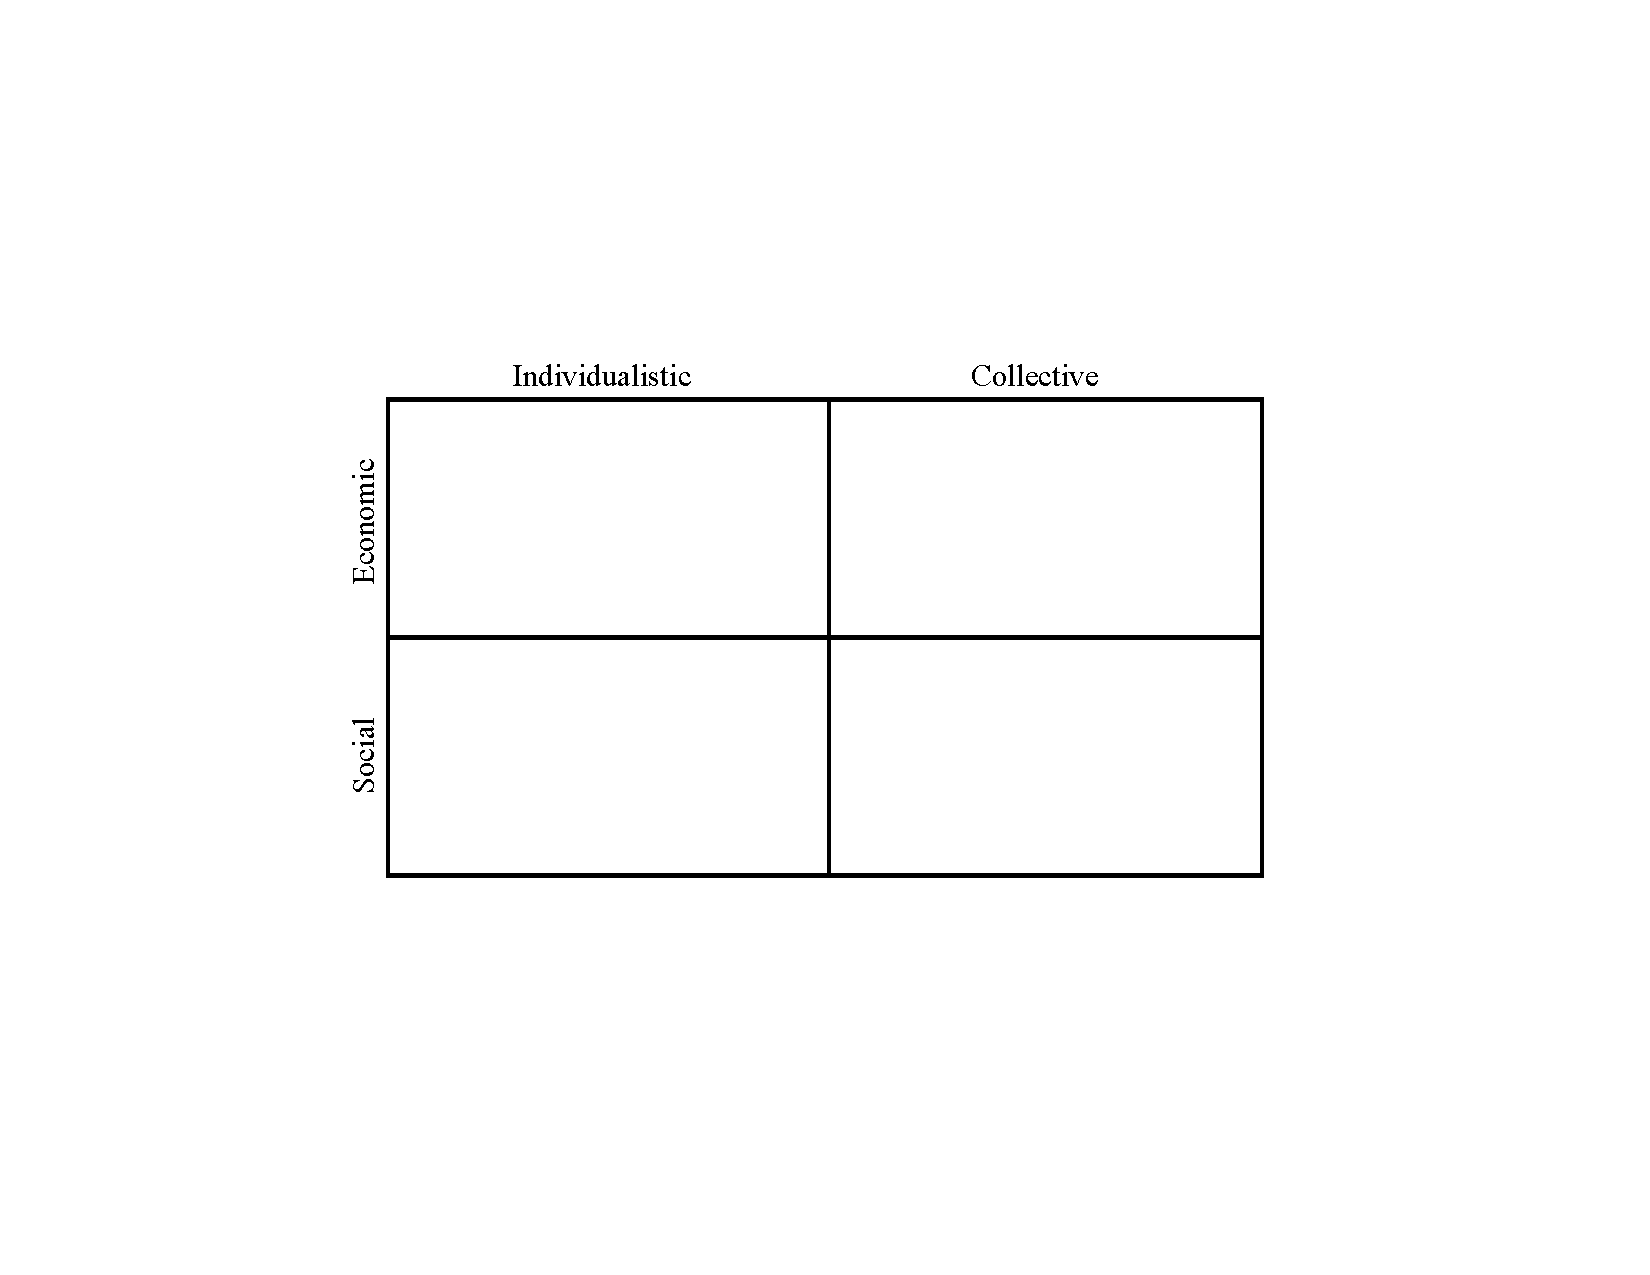
\includegraphics[width=0.75\linewidth]{figure_other/QuadTable}
\caption{Table for individualistic and collectivistic views on economic and social issues.}
\label{fig:table}
\end{figure}

% Need to refer to the figure. Need to harmonize/standardize terminology. I suggest ``individual'' and ``collective'' and the ``-ivistic'' ending.
% Need to note that these cut across, to some degree, the ``Christian'' axis. 

The economic and social aspects of sustainability are inextricably linked. Biblical teaching on money
and justice are often recognized as two sides of the same coin, for instance in Micah 2:1-2, where the unjust deeds that
are denounced are economic in nature. Biblical teaching on economics and justice tends not to be in terms of a
systematic, over-arching theory, but rather in terms of individual interactions.
One exception to this pattern is the Old Testament sabbatical/jubilee system of canceling debt and returning property. 
In modern economic terms, canceling debts and returning property would serve to minimize 
\emph{income inequality} and ensure that there was universal access to the \emph{means of production}.
% Insert Matt's really important comment here.

From the first chapter of Genesis, the call to stewardship has
been understood by Christians to include money. The power of earthly resources to accomplish ``heavenly things'' is made
explicit in the parable of the shrewd (or dishonest) manager in Luke 16. To this end, the great majority of the Bible's
teaching on money relates to generosity to the poor. Numerous Old and New Testament passages instruct God's faithful to
give generously to the poor, the disadvantaged, and the marginalized, where ``giving'' is some combination of money
(traditionally called ``alms''), material goods (such as food or clothing), and justice or fairness.

One branch of Christian thought views wealth itself as a root of evil. This view goes beyond merely \emph{love} money
being the root of evil (I Tim 6:10). Proponents of the view that money itself is a source of evil would point to Jesus
telling the rich young man to sell all his possessions and give to the poor and Jesus' further comment that it is easier
for a camel to go through the eye of a needle than for a rich man to enter the kingdom of God (Mt 19:16-30, Mk 10:17-31,
Luke 18:18-30). At the other end of the spectrum of Christian thought, worldly wealth is seen as God's blessing, even an
indication of his favor (in a more extreme version of this view).

In terms of modern economic views, Christians hold a wide range of positions. Some Christian traditions advocate a
communal economic arrangement, in imitation of the early church (Acts 2:42-46). Examples range monastic orders such as
might be found in Roman Catholic or Eastern Orthodox traditions to the Hutterite and Bruderhof communities, which come
from an Anabaptist tradition. At the other end of the economic spectrum, many Christians advocate for an economic system
based on individual ownership and freedom of enterprise. Some key verses that support a more individual view include the
comments ``Didn’t it belong to you before it was sold? And after it was sold, wasn’t the money at your disposal?'' (Acts
5:4) and Paul's instruction that we should work to eat (2 Thes 3:10) and to share with those in need (Eph 4:28).
Thus, Christians hold a range of views from economic thought from communalistic to individualistic.

Likewise, Christian social perspectives can stress individual freedom or collective behavior
A liberal approach to providing for poor widows would be represented by the instruction that widows should be 
provided for, first of all, from their own families (1 Tim 5:4). 
The collective approach is represented by the group effort of caring for widows at the beginning of Acts chapter 6.
Denominational polity is another example of the individual-to-collective spectrum.
At the individual end of the spectrum are ``independent'' churches that recognize no higher authority than the congregation itself.
In the middle are denominations that follow a presbyterian form of church 
government. The local church in the presbyterian system has some autonomy but within the constraints of the broader 
denominational structure. The local churches also have a voice in the operation of the collective. At the collective end of the spectrum 
are denominations that use an episcopal form of church government. Denominations with an episcopal polity operate in a very ``top down'' 
way.

We next show how the individualistic/collectivistic economic and social (that is, political) perspectives apply to a solving sustainability problems.

\subsection{Christian solutions to the tragedy of the commons}
\label{sec:totc}
The term ``tragedy of the commons'' was popularized by Hardin \autocite{Hardin68} 
and is used as a shorthand way of referring to
situations where there is equal and open access to a resource or pool of resources and it is in the rational self-interest of
every individual to maximize their use of the resource, even if this results in the net effect of destroying the
resource itself through over exploitation. This class of problems is recognized as ``having no technical solution.''
Instead, sustainable solutions are the result of social and/or economic policies. This section will examine several
Christian responses to the tragedy of the commons.

As originally stated, each herdsman had incentive to add more animals to his flocks grazing on the common land, since
the benefits (the extra animals) would accrue solely to him but the cost (degradation of the land) would be split between
all herders using the land for grazing. Moreover, since he knew that every other herder faced the same set of
incentives, it is rational to predict that the land will be ruined and that he should ``get while the getting is good.''
The ``tragedy'' lies in the ``remorseless working out of things.''

One collectivistic solution to the tragedy of the commons is for all of the animals grazing on the commons to be common
property. Every member of the community would receive an equal share of the common herd (for example, cash value of the
meat raised at the end of the year). It would thus be in every individual's self-interest to maximize the \emph{total}
output, not just their own output. An individualistic solution is to charge each herder an increasing amount of rent for
each additional animal placed on the common land, which would create a financial incentive for each herdsman to keep
only a reasonable number of animals on the common land. A liberal social solution would be for each herder to be allowed
only a limited number of animals on the common land. A collective solution would be where an authoritative governing
board is set up to administer the common land. The board decides how many animals total are allowed and what proportion
of that total is allocated to each individual herdsman.

As we'll see below, many sustainability challenges are wholly or partly ``without technical solution'' and we need
Christian approaches to solving these problems.

%
%Wealth is a sign of God's blessing. 
%Personal property. Western of ``Christian'' concepts.
%The Enlightenment and the concept of personal freedom.
%Development of corporations.
%Theology of saving. Commerce, banking, financial trading.
%Roman Catholic response(s) to communism?
%Who owns land? Labor? Capital?
%
%% Quote from Wikipedia on Distributionism 
%% https://en.wikipedia.org/wiki/Distributism
%Distributism is an economic ideology asserting that the world's productive assets should
%be widely owned rather than concentrated.[1] It was developed in Europe in the late 19th
%and early 20th centuries based upon the principles of Catholic social teaching, especially
%the teachings of Pope Leo XIII in his encyclical Rerum novarum (1891) and Pope Pius XI in
%Quadragesimo anno (1931).[2][3][4] It views both capitalism and socialism as equally
%flawed and exploitative, and it favors economic mechanisms such as small-scale
%cooperatives and family businesses, and large-scale anti-trust regulations.
%
%Some Christian Democratic political parties have advocated distributism in their economic
%policies.
% end quote

% In this issue, Nathan Schneider writes about Pope Francis’s economics. Here, he
% recommends five books of Catholic thought that display strikingly similar concerns to
% those of secular activists today. Each one emphasizes the wisdom of ordinary people. “In
% church each week,” Schneider says, “I learn Catholic economics from the diversity of
% classes and colors who meet under the image of an executed radical.”
%  https://www.thenation.com/article/classics-of-catholic-economics/

% from ENGR 184 lecture slides: 
% ``socially desirable and economically viable.''
% Economic: profit, cost savings, economic growth, R\&D
% Social: standard of living, education, community, equal opportunity. These combine to be business ethics, fair trade, women's rights.
% Economics refers to the whole community impact, not just a company's bottom line.
% social is fair business practices to labor and the community (whatever that means).
% Economics is the social science that seeks to describe the factors which determine the production, distribution, and consumption of goods and services.
% Food production, distribution, quality -- relates to land use and water consumption (3 models of agriculture: what's ``most efficient?'')

%Suffering and justice. Care for the poor. 
%Kings, democracy, dictators.
%What are the means of redress?
%Just war? just use of ``power?''
%Sphere sovereignty and the role of government? Church? family ... school...


%1%%%%%%%%%%%%%%%%%%%%%%%%%%%%%%%%%%%%%%%%%%%%%%%%%%%%%%%%%%%%
\section{Environmental} % == ``environmental stewardship'' ??
\label{sec:environmental}
%%%%%%%%%%%%%%%%%%%%%%%%%%%%%%%%%%%%%%%%%%%%%%%%%%%%%%%%%%%%%%

% These would still be good to do.

%\ins{Add first action for sustainability? The weakness or pitfall of each approach. (for instance, lack of information?)
%Need to add in for each worldview, discussion question 13, what is the purpose of the natural world?
%Re-look for scriptural references and include in the first paragraph (or a 2nd paragraph).
%Then say how each tradition takes something different from the same scriptural references.}

The book \emph{Ecologies of Grace} \autocite{Jenkins:2008}
provides a topology of Christian thought regarding the 
nonhuman creation and the
environmental aspect of sustainability.
He identifies three schools of thought:
stewardship, 
eco-justice, and 
ecological spirituality,
which loosely correspond to 
Reformed (or evangelical protestant), 
Roman Catholic, and 
Eastern Orthodox 
traditions.
To Jenkins' three, we add a fourth:
consumptive economic prosperity and
the conservative evangelical tradition. 
These four schools of thought 
span a wide range of Christian stances toward the nonhuman creation
and 
consequently outline a range of possibilities 
for Christian responses to environmental issues
and environmental sustainability concerns more broadly.
One way to begin unpacking the four schools of thought 
is to identify a keyword for each:
\emph{redemption} for stewardship, 
\emph{sanctification} for eco-justice,
\emph{deification} for ecological spirituality, and
\emph{resilience} for consumptive economic prosperity.

%..............................
\paragraph{Redemption} 
\label{sec:redemption}
%..............................

The stewardship school of thought in the Reformed tradition
emphasizes that all of human existence
is a response to God's redemptive acts
and God's providence to humans.
Knowing God leads to vocational responsibility 
to care for nonhuman creation,
the means by which God provides for humankind  % ==== telos?!
% For some reason, we need to include this citation twice to get both author and page number to appear.
(\textcite{Jenkins:2008} \textcite[19]{Jenkins:2008}). 
Thus, all human work to care for the creation 
is seen as service to the Creator
out of gratitude for redemption (\textcite{Jenkins:2008} \textcite[77]{Jenkins:2008}).
\emph{Earthkeeping} \autocite{Wilkenson:1980aa} provides a cogent summary
of the importance of redemption for Reformed Christians doing creation care.

The idea of stewardship is a reaction against themes of human dominion over the nonhuman creation
that emerge from some interpretations of the creation stories in Genesis.
Christians in this tradition are inspired by an interpretation of Gen~1:26–28 in which 
``the proper exercise of dominion yields shalom: the flourishing of all creation'' \autocite{BoumaPrediger:2019}.
As such, the first order of business for stewardship-minded Christians
is to act as shalom-building caretakers of God's creation.

%..............................
\paragraph{Sanctification} 
\label{sec:sanctification}
%..............................

The eco-justice school of thought in the Roman Catholic tradition
emphasizes that God's grace reveals the creation's 
inherent integrity \autocite[19]{Jenkins:2008}, 
giving it natural value and inherent moral standing~\autocite{Joldersma:2019}. 
Thus, Christians must respect creation's inherent value and 
respond to its moral standing in all activities.
If the nonhuman creation can't speak for itself, 
we must speak for it and defend it when necessary.

The \emph{Laudato Si} encyclical \autocite{Pope-Francis:2015aa} 
is a clear enunciation of Roman Catholic thought
on environmental sustainability issues.
In it, Pope Francis portrays the nonhuman creation as a
``sister with whom we share our life and a beautiful mother who opens her arms to embrace us''
(\textcite{Pope-Francis:2015aa} \textcite[3]{Pope-Francis:2015aa}).
However, our sister and mother
``cries out to us because of the harm we have inflicted on her 
by our irresponsible use and abuse of the goods with which God has endowed her''
(\textcite{Pope-Francis:2015aa} \textcite[3]{Pope-Francis:2015aa}).
With this framing, the Holy Father evokes centuries of Catholic social teaching
about the need to support the oppressed, the poor, and the vulnerable.
Christians in the eco-justice tradition would point to the beatitudes (Lk 6) 
for reminders of the inherent value of those who are oppressed.
The first order of business for eco-justice-minded Christians
is to bring justice to the nonhuman creation, to right the wrongs
of abuse that humans have heaped upon the nonhuman creation.
\ins{this is the ends. What about the means?}

%..............................
\paragraph{Deification} 
\label{sec:deification}
%..............................

The deification school of thought in the Eastern Orthodox tradition
highlights the union between all of creation and God.
This view holds that there is a radical, integral relationship between humans and 
the nonhuman creation~\autocite[93]{Jenkins:2008}.

The speech ``To Commit a Crime Against the Natural World Is a Sin'' 
\autocite[133-136]{Bartholomew-I-of-Constantinople:2011aa}
provides an excellent summary of the Eastern Orthodox view
on the nonhuman creation.
In it, Bartholomew states,
``at the heart of the relationship between man and environment 
is the relationship between human beings.
As individuals, we live not only in vertical relationships to God 
and horizontal relationships to one another, but 
also in a complex web of relationships that extend throughout
our lives, our cultures, and the material world.''
(\textcite{Bartholomew-I-of-Constantinople:2011aa} 
\textcite[133--134]{Bartholomew-I-of-Constantinople:2011aa})
Thus, any harm done to the nonhuman creation is a harm done to other human being. 
And the first order of business for Christians in the ``ecological spiritualities'' mindset %%%%%%%%%%%%%% why plural?
is asceticism, self-restraint for the good of the nonhuman creation and for others. % why the comma?s
Asceticism will lead to practices that look much like conservation of the nonhuman creation.

%..............................
\paragraph{Resilience} 
\label{sec:resilience}
%..............................

The resilience school of thought in the conservative evangelical tradition
holds that the nonhuman creation is resilient, robust, and self-correcting.
Furthermore, its well-being is assured by God because part of the ``goodness'' that God design into the world is robustness to human action.
God is always in control.
In this school of thought, human well-being is paramount. 
Thus, humans are to be consumers of the nonhuman creation 
to provide economic prosperity and
lift people out of poverty.
Documents from the Cornwall Alliance 
provide a summary of conservative evangelical thinking on creation care issues
\autocite{Cornwall:2006aa}.

% *** Here is a URL that shows how to convert a .csv file into a LaTeX table.
%
% \url{https://www.latex-tutorial.com/tutorials/pgfplotstable/}
%
% Here is a link to the Google sheet.
%
% {\tiny \url{https://docs.google.com/spreadsheets/d/1OD7LFbCU0Rdv3-vAM0MbIBd4hkEwxwY2FtP0XfvAU_M/edit#gid=0}}

\section{How Christian Views on Eschatology and the \emph{telos} of Creation Affect Sustainability}
Some info on these topics in the ENGR 184 lecture slides.

%%%%%%%%%%%%%%%%%%%%%%%%%%%%%%%%%%%%%%%%%%%%%%%%%%%%%%%%%%%%%%
\section{Application: Evaluating a proposed ban on fossil-fueled personal transportation}
\label{sec:personal_transportation}
%%%%%%%%%%%%%%%%%%%%%%%%%%%%%%%%%%%%%%%%%%%%%%%%%%%%%%%%%%%%%%

\ins{How does this get us closer to being able to make sustainability choices?}

% needs to somehow address the framework by which we make choices. I want to get at the utter failure of current and past modes of thinking
% in allowing us to address sustainability-related questions.
Far from being esoteric or merely philosophical, 
the impact of worldview on sustainability issues and behavioral choices 
is both crucially important and entirely practical. 
Thus, it is \emph{essential} that engineers consider worldviews
when examining choices and tradeoffs related to sustainability.
This section considers, as a practical example, the effects of different Christian approaches
to the economy and societal structures (Section~\ref{sec:economic}) and
to the nonhuman creation (Section~\ref{sec:environmental})
on a sustainability-related policy question, 
namely whether to ban vehicles for personal transportation.

In 2017, the United States emitted 5.14 billion metric tons equivalent of greenhouse gases, 
of which, about 1.8 billion tons (35\%) were from petroleum used for transportation \cite{EIA2017}.
\b{Consider a proposed ban on personal transportation vehicles the burn fossil fuels.}
Commercial vehicles are not addressed by the proposed ban. % is that fair? what about rental cars?

The alternative to the proposed ban is to do nothing. 
Under this ``null hypothesis,'' 
significant amounts of greenhouse gasses would be added to the atmosphere 
at ever-increasing rates. \ins{Do we need to explain ever-increasing rates?}
Enacting the proposed ban would eliminate a (major) category 
of greenhouse gas emissions and 
would be a step on the road toward sustainability
and would, presumably, avoid future costs for climate change adaptation.
However, the proposed ban would involve massive monetary costs in the near-term. 
Billions of dollars per year would be required. 
One estimate \ins{citation needed} is that it would require between 7 and 14\% of GDP annually 
over 20 years to achieve a fully-renewable transportation infrastructure.

Emplacing a fully-renewable transportation infrastructure 
would displace or require thorough transformation of many existing industries, including 
the automobile industry, 
the liquid petroleum distribution industry, and
the electricity generation and distribution industries,
to name a few.
Disruptions in those industries 
would cause massive social disruptions 
as jobs are lost.
%Therefore, a large-scale job retraining effort would be necessary.   % Non sequitur.

The proposed ban would have massive implications for real estate values 
and patterns of land use. 
Presumably, rural living would be much more difficult if the proposal were enacted,
whereas urban dwellers could avail themselves of extensive public transit networks.


%++++++++++++++++++++++++++++++
\subsection{Evaluating tradeoffs}
\label{sec:evaluating_tradeoffs}
%++++++++++++++++++++++++++++++

Implementing the proposed ban on fossil-fueled personal transport vehicles
will involve tradeoffs among the dimensions of sustainability, 
environmental, economic, and social factors.
Decisions on tradeoffs are necessarily informed by worldviews,
many of which are briefly described 
in Sections~\ref{sec:economic} and~\ref{sec:environmental}.
In this subsection, 
we use the proposed ban to explore how Christian worldviews matter 
for tradeoffs when sustainability issues are at stake.
That is, how do each of the Christian traditions 
\ins{(Is Christian traditions the right way to discuss these ideas?)} 
discussed in this paper 
evaluate tradeoffs among environmental, social, and economic factors?
We briefly summarize each tradition below.
\ins{again, maybe want to merge with sections above to avoid repetition. What are the weaknesses of each approach?}

% I'm going to recommend only associating denominations to worldviews once.
% Let's make the the paragraphs a bulleted list instead. Condense each paragraph to a bullet.
\begin{itemize}
\item Those who hold \emph{individualistic} economic and social viewpoints would be unlikely to support a 
ban on personal vehicles that burn fossil fuels. There should be freedom for each individual to make their own
choice about how to travel. Instead, each individual should respond to incentives to achieve a collective good. 

\item Those who hold to a \emph{collective} approach to economic and social aspects of sustainability might welcome a
ban on fossil-fuel burning personal transportation as an expedient way of achieving reduced carbon emissions or might favor other 
policies as being ``better'' or more efficient.

\item The \emph{stewardship} viewpoint acknowledges that tradeoffs %% called ``Redemption''?
are present in every policy and in every decision. 
So, in an engineering sense, 
Christian environmental stewardship could be considered an optimization problem
in which policies that bring about the most good 
are to be preferred.
\ins{The ban on fossil-fuel-fired personal transportation would be critiqued based on the \emph{process} by which
the ban is enacted. Were all voices heard? Was the assessment of tradeoffs accurate?}
Who decides what goods matter most is important, and 
all voices should be heard on this matter.
Ignoring or disregarding voices is dangerous,
since injustices could result. %need perfect economic and environmental information?
Humans will be persuaded on the right course of action
for sustainability policies by weighing the tradeoffs 
among environmental, economic, and social factors.
% I think a lot of the above verbage could move back to the Environmental section.
\ins{Here is an example of where imperfect information, in both an engineering sense and an economic sense, would bite you big time.}
%The stewardship approach emphasizes the human responsibility 
%to care for the nonhuman creation
%as a response to God's redemptive actions.

\item The {eco-justice} point of view % SANCTIFICATION?
would weigh the environmental justice of the proposed ban (good for the natural world) against the possible 
economic injustice of depriving the poor of transportation. They would be more likely to support the ban if it
were accompanied by a robust and reliable system of public transportation.
% is based upon the moral standing of the nonhuman creation,
% meaning that the nonhuman creation itself must be given a voice.  %<<<<<<<<<<< Move these lines (and below?) to section 4?
%To properly evaluate sustainability tradeoffs,
%someone must be empowered to speak for the nonhuman creation and 
%give voice to unjust and unfair aspects of policies and decisions
%that have implications for sustainability and the nonhuman creation.
%Humans will pursue the right course of action on sustainability issues
%when someone speaks eloquently and forcefully for the 
%those who can't speak for themselves, including the nonhuman creation. 

\item In \emph{ecological spirituality} tradeoffs between the environmental and economic and social realms of sustainability
fade into the background. Any good done to the environment is a good done to humans, 
and praiseworthy. Thus, they would favor a ban on fossil-fuel burning personal vehicles.

% the radical connection between 
%the creator and the creation.
%Consequently, and by virtue of both owing their existence to the creator, 
%there is a radical connectedness among all human and nonhuman creatures in the creation.
%Because of this radical connection between humans and the nonhuman creation, 
%any good done to the environment is a good done to humans, 
%and praiseworthy. 
%Conversely, any environmental harm is a harm to humans and sinful. 
%We should always be doing right by ourselves and the environment 
%to please the God of us all.
%In ecological spirituality, 
%tradeoffs between the environmental and social realms of sustainability
%fade into the background.
%And because the economy is a way of organizing social relationships and structures,
%tradeoffs between the environmental and economic are minimized, too.

\item People with the \emph{consumptive economic prosperity} worldview
will note that any environmental degradation caused by humans will be fixable,
given sufficient economic resources and the guidance of the free market's invisible hand.
A ban on fossil-fueled personal transport vehicles 
will likely lead to decreased economic prosperity,
because some people will no longer be able to work,
commute times will increase for others, and 
commerce will slow. 
A reduction in economic prosperity will, ultimately, be bad for the environment, because
we will have fewer economic resources with which to address environmental damage.
Thus, they would be unlikely to support the proposed ban on personal transportation vehicles.
\end{itemize}

%++++++++++++++++++++++++++++++
\subsection{A critique of the proposed ban} %             I'm not sure we need this section. Could we blend this into the Conclusions instead?
\label{sec:conundrum}
%++++++++++++++++++++++++++++++

\paragraph{Alternatives} It may be possible to incentivize low-impact vehicles, including bicycles and renewable-energy vehicles.
Policies to incentivize adoption of 
mass-transit (subways and buses) or shared transit (Lyft and Uber)
could allow societies to meet transport needs with significantly less environmental impact 
per person-km.

%But tradeoffs exist. 
\paragraph{Tradeoffs} There are financial costs to changing the transportation infrastructure to low-impact vehicle technologies
or away from personal to mass-transit solutions. 
There will be social costs to changing the transportation infrastructure as well.
Relationships and employment may be disrupted by changes in the availability of personal transport vehicles,
especially if substitutes are of lesser quality or availability.
Converting to a renewable-energy personal transportation infrastructure 
might imply land-use changes, 
requiring significant amounts of space for solar and wind renewable electricity production,
not to mention storage needs. 
Will land-use changes impinge on the ``freedom'' or rural life 
or increase the density of urban living?

%..............................
\paragraph{How might Christian worldviews shape perceptions of these tradeoffs?} %  The text in this section is mostly repeated from the sections above. Delete and/or blend into the conclusions.
%..............................

Perceptions of the desirability and advisability of choices implied by these tradeoffs 
will be shaped by the Christian worldviews discussed above.

For example, stewardship concerns may indicate deep study of alternatives, 
weighing weigh costs and benefits in the environmental, economic, and social realms
to discover the best way to manage the human and nonhuman elements of creation.
Study and deliberation will be in order as debates over the numeraire for comparisons arise. 
Those informed by an eco-justice worldview may want to evaluate 
differential benefits and costs of a transportation system overhaul.
To whom will benefits and costs accrue? 
Which people groups will benefit most and least? 
Which portions of the nonhuman creation will benefit or be harmed? 
Those in the deification school of thought might be concerned 
about loss of quality of personal connections 
among people due to transportation system disruption
and advocate for policies that ensure transportation system changes 
are coupled with ways to increase the connectedness that people
feel toward the nonhuman creation.
Those with a resilience mindset may be likely to disfavor 
large-scale changes to the transportation infrastructure 
on the grounds that the financial cost of a transportation system overhaul would be burdensome,
without much regard for any environmental benefits, 
because the Earth system is resilient anyway.



% Maybe different rules for different places?
% Techno-optimism (technocism?)
% posits there is a way to solve all problems with sufficiently advanced technology.
% What would be the (socialism?) way?---there's a way to solve every problem
% with a sufficiently advanced society.




%%%%%%%%%%%%%%%%%%%%%%%%%%%%%%%%%%%%%%%%%%%%%%%%%%%%%%%%%%%%%%
\section{Conclusions}
\label{sec:conclusions}
%%%%%%%%%%%%%%%%%%%%%%%%%%%%%%%%%%%%%%%%%%%%%%%%%%%%%%%%%%%%%%

% one conclusion that we've talked about is the need for a theology that addresses corporate sin/responsibility for the environment.
% How does, for instance, covenant theology lead us to sustainability?

The purpose of this paper is to explore how
Christian worldviews matter 
when sustainability issues are at stake. 
The example discussed in Section~\ref{sec:personal_transportation} shows that
Christian worldviews can and do 
both inform responses to sustainability issues
and affect assessments of policy tradeoffs.

In reviewing Sections~\ref{sec:environmental}--\ref{sec:personal_transportation},
it becomes clear that there is an urgent need for a theology 
that addresses human effects on the nonhuman creation.
This theology should provide guidance for daily life and 
for corporate decision- and policy-making on several axes:
economic gain vs.\ environmental harm, 
individual harm vs.\ corporate good, 
benefits to the current generation vs.\ future generations,
environmentally harmful but convenient solutions vs.\ environmentally benign but inconvenient solutions, 
dollar-quantifiable goods and harms vs.\ non-quantifiable goods and harms,
costs and benefits that accrue to an individual vs.\ a group
or a group vs.\ an individual, etc.

Indeed, there is much work to be done.

\printbibliography
\end{document}